\documentclass{standalone}
\usepackage{tikz}
\usetikzlibrary{patterns, positioning}
\usepackage[sfdefault]{ClearSans} %% option 'sfdefault' activates Clear Sans as the default text font
\usepackage[T1]{fontenc}

\begin{document}
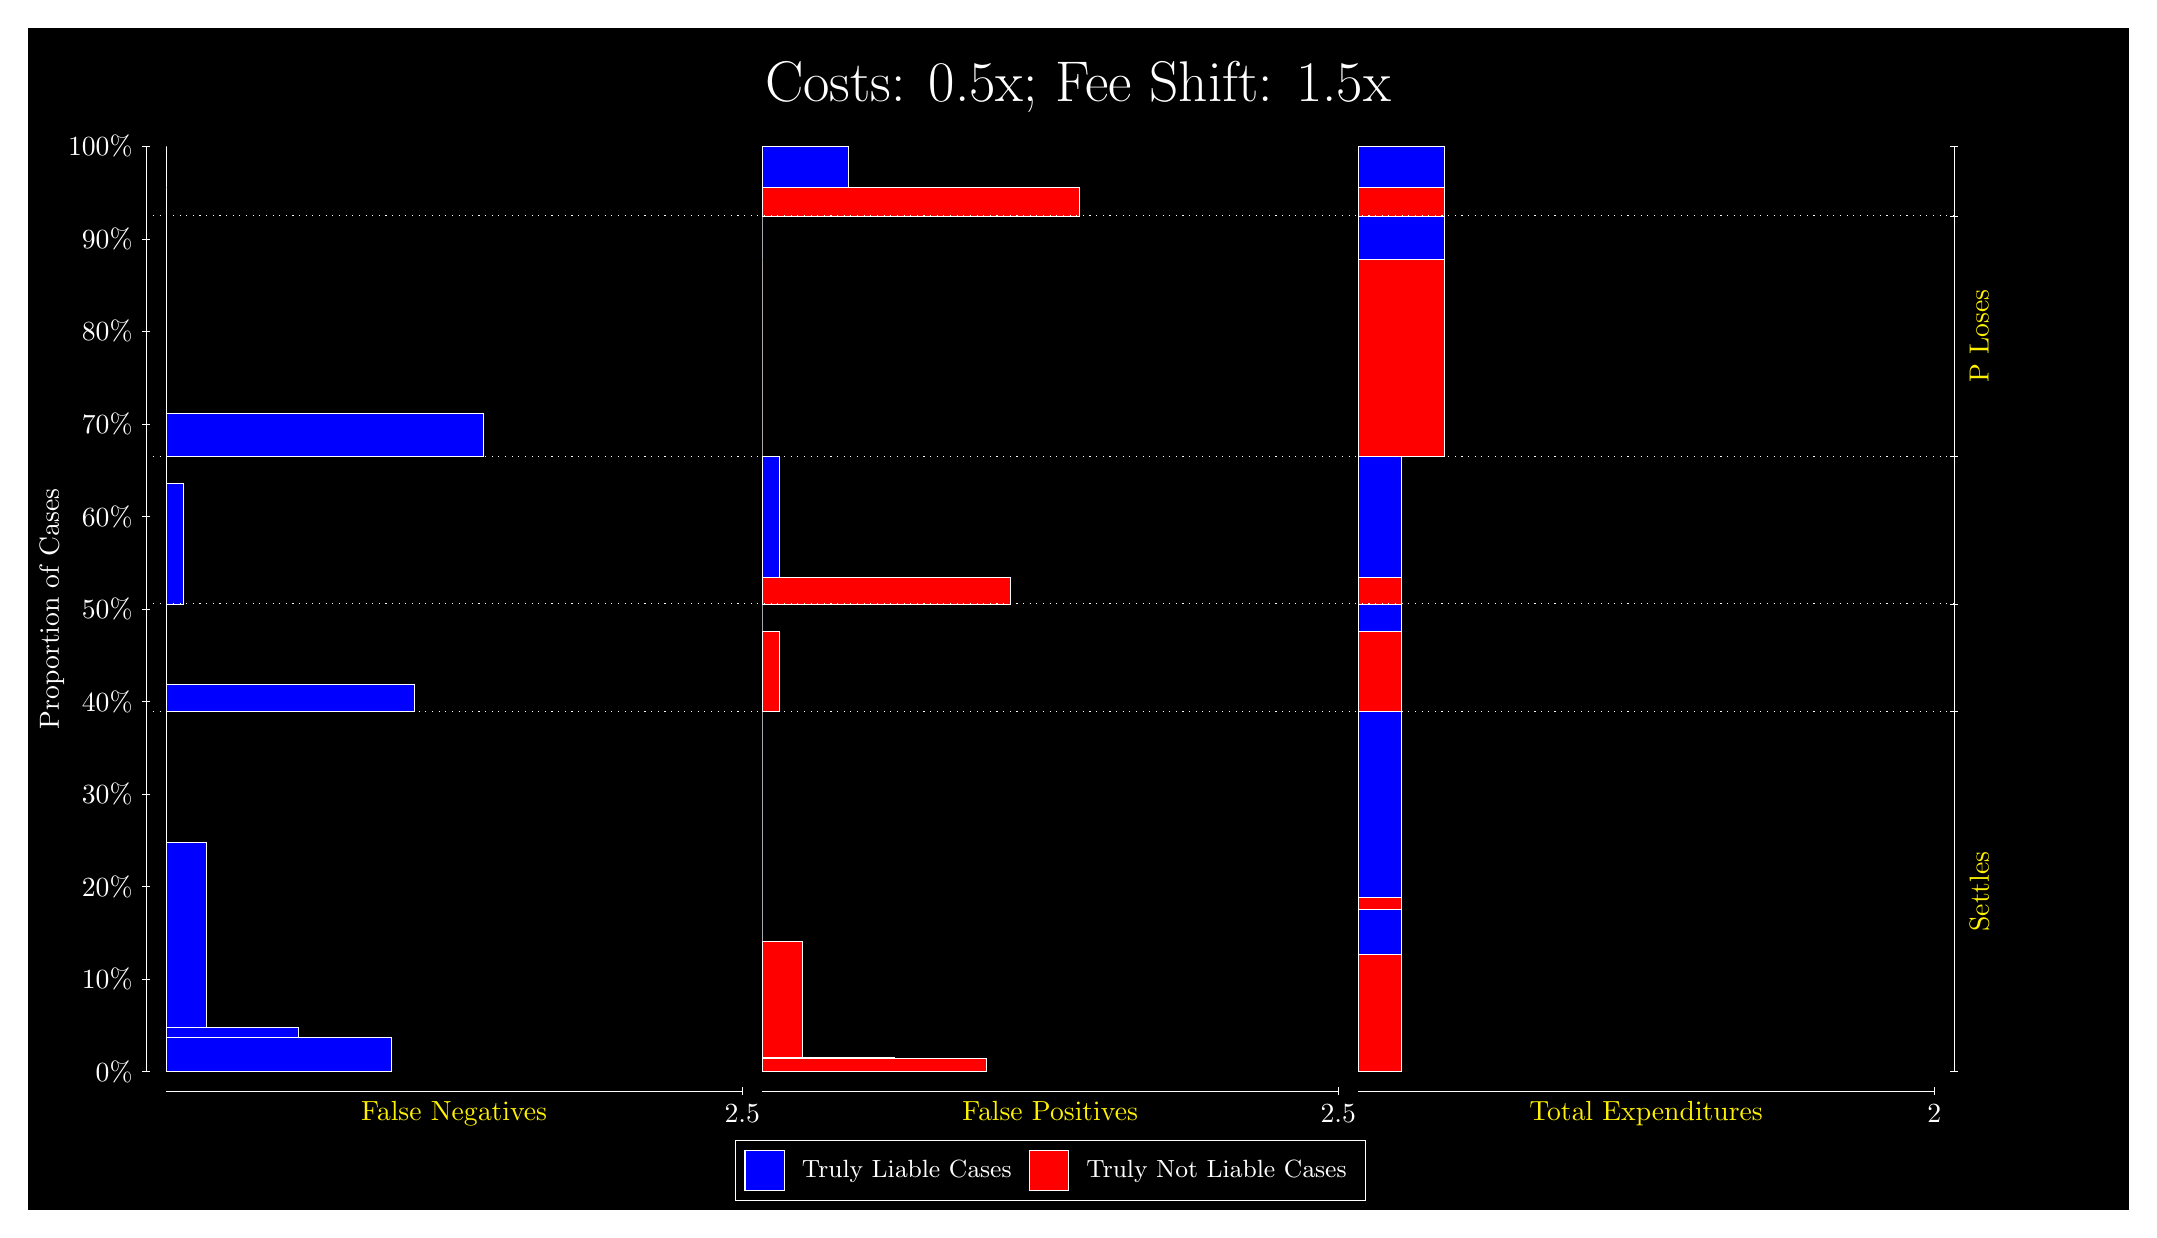
\begin{tikzpicture}
\draw[fill=black] (0,0) rectangle (26.667,15);
\draw[text=white] (0,13.5) rectangle (26.667,15) node[midway] {\huge Costs: 0.5x; Fee Shift: 1.5x};
\draw[white, very thin] (1.5,1.75) -- (1.5,13.5);
\node[rotate=90, text=white, anchor=center] at (0.3, 7.625) {Proportion of Cases};
\draw[white, very thin] (1.45,1.75) -- (1.55,1.75);
\node[text=white, anchor=east] at (1.45, 1.75) {0\%};
\draw[white, very thin] (1.45,2.925) -- (1.55,2.925);
\node[text=white, anchor=east] at (1.45, 2.925) {10\%};
\draw[white, very thin] (1.45,4.1) -- (1.55,4.1);
\node[text=white, anchor=east] at (1.45, 4.1) {20\%};
\draw[white, very thin] (1.45,5.275) -- (1.55,5.275);
\node[text=white, anchor=east] at (1.45, 5.275) {30\%};
\draw[white, very thin] (1.45,6.45) -- (1.55,6.45);
\node[text=white, anchor=east] at (1.45, 6.45) {40\%};
\draw[white, very thin] (1.45,7.625) -- (1.55,7.625);
\node[text=white, anchor=east] at (1.45, 7.625) {50\%};
\draw[white, very thin] (1.45,8.8) -- (1.55,8.8);
\node[text=white, anchor=east] at (1.45, 8.8) {60\%};
\draw[white, very thin] (1.45,9.975) -- (1.55,9.975);
\node[text=white, anchor=east] at (1.45, 9.975) {70\%};
\draw[white, very thin] (1.45,11.15) -- (1.55,11.15);
\node[text=white, anchor=east] at (1.45, 11.15) {80\%};
\draw[white, very thin] (1.45,12.325) -- (1.55,12.325);
\node[text=white, anchor=east] at (1.45, 12.325) {90\%};
\draw[white, very thin] (1.45,13.5) -- (1.55,13.5);
\node[text=white, anchor=east] at (1.45, 13.5) {100\%};

\draw[white, very thin] (24.457,1.75) -- (24.457,13.5);
\draw[white, very thin] (24.407,1.75) -- (24.507,1.75);
\node[anchor=west] at (24.407, 1.75) {};
\draw[white, very thin] (24.407,6.3206) -- (24.507,6.3206);
\node[anchor=west] at (24.407, 6.3206) {};
\draw[white, very thin] (24.407,7.6904) -- (24.507,7.6904);
\node[anchor=west] at (24.407, 7.6904) {};
\draw[white, very thin] (24.407,9.5579) -- (24.507,9.5579);
\node[anchor=west] at (24.407, 9.5579) {};
\draw[white, very thin] (24.407,12.616) -- (24.507,12.616);
\node[anchor=west] at (24.407, 12.616) {};
\draw[white, very thin] (24.407,13.5) -- (24.507,13.5);
\node[anchor=west] at (24.407, 13.5) {};

\draw[white, very thin, fill=blue] (1.75,1.75) rectangle (4.6044,2.1787);
\draw[white, very thin, fill=blue] (1.75,2.1787) rectangle (3.4333,2.3139);
\draw[white, very thin, fill=blue] (1.75,2.3139) rectangle (2.2623,4.6671);
\draw[white, very thin, fill=red] (1.75,4.6671) rectangle (1.75,6.3206);
\draw[white, very thin, fill=blue] (1.75,6.3206) rectangle (4.8971,6.6672);
\draw[white, very thin, fill=red] (1.75,6.6672) rectangle (1.75,7.6904);
\draw[white, very thin, fill=blue] (1.75,7.6904) rectangle (1.9696,9.2215);
\draw[white, very thin, fill=red] (1.75,9.2215) rectangle (1.75,9.5579);
\draw[white, very thin, fill=blue] (1.75,9.5579) rectangle (5.7754,10.112);
\draw[white, very thin, fill=red] (1.75,10.112) rectangle (1.75,12.616);
\draw[white, very thin, fill=red] (1.75,12.616) rectangle (1.75,12.974);
\draw[white, very thin, fill=blue] (1.75,12.974) rectangle (1.75,13.5);
\draw[white, very thin, fill=red] (9.3189,1.75) rectangle (12.173,1.913);
\draw[white, very thin, fill=red] (9.3189,1.913) rectangle (11.002,1.9258);
\draw[white, very thin, fill=red] (9.3189,1.9258) rectangle (9.8312,3.4034);
\draw[white, very thin, fill=blue] (9.3189,3.4034) rectangle (9.3189,6.3206);
\draw[white, very thin, fill=red] (9.3189,6.3206) rectangle (9.5384,7.3437);
\draw[white, very thin, fill=blue] (9.3189,7.3437) rectangle (9.3189,7.6904);
\draw[white, very thin, fill=red] (9.3189,7.6904) rectangle (12.466,8.0268);
\draw[white, very thin, fill=blue] (9.3189,8.0268) rectangle (9.5384,9.5579);
\draw[white, very thin, fill=red] (9.3189,9.5579) rectangle (9.3189,12.061);
\draw[white, very thin, fill=blue] (9.3189,12.061) rectangle (9.3189,12.616);
\draw[white, very thin, fill=red] (9.3189,12.616) rectangle (13.344,12.974);
\draw[white, very thin, fill=blue] (9.3189,12.974) rectangle (10.417,13.5);
\draw[white, very thin, fill=red] (16.888,1.75) rectangle (17.437,3.2404);
\draw[white, very thin, fill=blue] (16.888,3.2404) rectangle (17.437,3.8043);
\draw[white, very thin, fill=red] (16.888,3.8043) rectangle (17.437,3.9673);
\draw[white, very thin, fill=blue] (16.888,3.9673) rectangle (17.437,6.3206);
\draw[white, very thin, fill=red] (16.888,6.3206) rectangle (17.437,7.3437);
\draw[white, very thin, fill=blue] (16.888,7.3437) rectangle (17.437,7.6904);
\draw[white, very thin, fill=red] (16.888,7.6904) rectangle (17.437,8.0268);
\draw[white, very thin, fill=blue] (16.888,8.0268) rectangle (17.437,9.5579);
\draw[white, very thin, fill=red] (16.888,9.5579) rectangle (17.986,12.061);
\draw[white, very thin, fill=blue] (16.888,12.061) rectangle (17.986,12.616);
\draw[white, very thin, fill=red] (16.888,12.616) rectangle (17.986,12.974);
\draw[white, very thin, fill=blue] (16.888,12.974) rectangle (17.986,13.5);
\draw[white, dotted] (1.5,6.3206) -- (24.457,6.3206);
\draw[white, dotted] (1.5,7.6904) -- (24.457,7.6904);
\draw[white, dotted] (1.5,9.5579) -- (24.457,9.5579);
\draw[white, dotted] (1.5,12.616) -- (24.457,12.616);
\draw[white, very thin] (1.75,1.5) -- (9.0689,1.5);
\node[text=yellow, anchor=north] at (5.4094, 1.5) {False Negatives};
\draw[white, very thin] (9.0689,1.45) -- (9.0689,1.55);
\node[text=white, anchor=north] at (9.0689, 1.45) {2.5};

\draw[white, very thin] (9.3189,1.5) -- (16.638,1.5);
\node[text=yellow, anchor=north] at (12.978, 1.5) {False Positives};
\draw[white, very thin] (16.638,1.45) -- (16.638,1.55);
\node[text=white, anchor=north] at (16.638, 1.45) {2.5};

\draw[white, very thin] (16.888,1.5) -- (24.207,1.5);
\node[text=yellow, anchor=north] at (20.547, 1.5) {Total Expenditures};
\draw[white, very thin] (24.207,1.45) -- (24.207,1.55);
\node[text=white, anchor=north] at (24.207, 1.45) {2};

\node[text=yellow, centered, rotate=90] at (24.777, 4.0353) {Settles};


\node[text=yellow, centered, rotate=90] at (24.777, 11.087) {P Loses};


\draw (12.978300999999998,1.5) node[draw=none] (baseCoordinate) {};
\begin{scope}[align=center]
        \matrix[scale=0.5, draw=white, below=0.5cm of baseCoordinate, nodes={draw}, column sep=0.1cm]{
            \node[rectangle, draw, minimum width=0.5cm, minimum height=0.5cm, fill=blue] {}; &
            \node[draw=none, font=\small, text=white] (B) {Truly Liable Cases}; &
            \node[rectangle, draw, minimum width=0.5cm, minimum height=0.5cm, fill=red] {}; &
            \node[draw=none, font=\small, text=white] (B) {Truly Not Liable Cases}; \\
            };
\end{scope}

\end{tikzpicture}
\end{document}